\chapter{System Maintenance}

\section{Environment}

\subsection{Software}

The following is the software used during my implementation.

\begin{itemize}
\item Python 3.3 and 3.4
\item IDLE
\item PyQt 4
\item SQLite 3
\item SQLite Inspector
\item SQLite Database Browser
\item Matplotlib
\item Adobe Photoshop CS5
\item cx\_Freeze
\end{itemize}

\subsection{Usage Explanation}

\begin{center}
    \begin{tabular}{|p{4cm}|p{6cm}|}
        \hline
        \textbf{Test Series} & \textbf{Purpose of Test Series} \\ \hline
        Python 3.3 and 3.4 & Used as my programming language to produce my system. I have chosen this language as I have been learning it in class for the past two years \\ \hline
        IDLE & I used this software as the developing environment. It was included with Python and has been the environment I have been using in classes so I am familiar with it. This made implementation easier\\ \hline
        PyQt 4 & Used to create the graphical user interface for my program \\ \hline
        SQLite 3 & This was used to access my database in order to extract and store information \\ \hline
        SQLite Inspector & This software allowed me to browse the database file when implementing the system. It was used to check data was being added, removed and changed correctly if accessed from inside the system. \\ \hline
        SQLite Database Browser & This program is similar to the inspector but was downloaded when I was working on my Macbook (rather than my computer). It performs the exact same task of viewing data in the database file. \\ \hline
        Matplotlib & This allows for extracting data from the database to produce graphs \\ \hline
        Adobe Photoshop CS5 & Used for creating the splash screen and adding transparency to arrows \\ \hline
        cx\_Freeze & Used in order to compile my system into an executable file (and windows installer) so it can be run by the user easily \\ \hline
    \end{tabular}
\end{center}

\subsection{Features Used}

\begin{center}
    \begin{tabular}{|p{4cm}|p{6cm}|}
        \hline
        \textbf{Test Series} & \textbf{Purpose of Test Series} \\ \hline
        Python 3.3 and 3.4 & Python provided me with the features needed to create my program in both CLI and GUI form. Python allows modules to be imported from elsewhere such as matplotlib (see below).  \\ \hline
        IDLE & IDLE is an environment specifically for Python and was used to create and run the code. The syntax highlighting that IDLE uses made implementing the program easier. \\ \hline
        PyQt 4 & A lot of features were used of PyQt such as stacked widgets, main windows and widgets. \\ \hline
        SQLite 3 & SQLite3 is essentially a simplified version of MySQL and included all of the functions I needed to deal with databases in my system. One of the features that was especially important was enforcing referential integrity which ensured that foreign keys matched existing primary keys.  \\ \hline
        SQLite Inspector & The execute feature was used to debug my SQL, this allowed me to test queries before they were ran in Python  \\ \hline
        SQLite Database Browser & I used this program for the same features as the Inspector shown above.   \\ \hline
        Matplotlib & The module from marplotlib known as 'Pylab' was used to create my graph, more specifically it was used to create a bar chart with axes titles.  \\ \hline
        Adobe Photoshop CS5 & The magic wand tool was used to remove image backgrounds (making them transparent), layering and selection tools were also used to create and edit images. \\ \hline
        cx\_Freeze & This software allowed me to compile my final system into a executable which will allow the user to simply double click the file to run the program. However I also used cx\_Freeze to produce an installer that will take the user through a step-by-step installation process and create a directory that the executable is stored in, this will also include all the extra files (pictures and database) \\ \hline
    \end{tabular}
\end{center}

\section{System Overview}

\subsection{Logins}

This part of the system will prevent any unauthorised access to the system. It will check the username and password input and compare it with usernames (primary keys in the database) and passwords stored in a database file. If the details match, the user will gain access to the relevant part of the system and the correct QMainWindow will appear. The system runs with access restrictions therefore usernames will have certain access levels attached to them which are (in order of access rights) Admin, Manager or Staff. If the username/password combination does not match a error will appear asking the user to re-enter the information until it is correct. There is also a "forgotten username or password" button to allow users to send emails to IT staff from inside the system which will request a password retrieval. All staff have the same email host (Volac.com) therfore I will be able to use the correct SMTP server when the system is given to my client. Currently, for testing purposes, the SMTP sever is "Live.com" this can easily be changed when the client uses the system.

\subsection{The Graphical User Interface}

The whole system is built with a graphical user interface (GUI) to make sure it is professional and user friendly. The GUI contains many different features including:
\begin{itemize}
\item Toolbar icons and menu bars for navigational purposes
\item Images to improve to overall look of the system
\item File browsing to choose the database
\item Line edits and combo boxes to allow a user friendly input of data
\item Labels for certain parts of the system to tell users what interface they are currently viewing
\item Stylesheets to improve the overall look and to match company website colours
\end{itemize}

\subsection{Open Database Interface}

The admin main menu will provide a button that will take the user to the 'Open Database' interface. This will most likely be the most used interface on the entire system because this is where IT Staff can add, remove and edit records on the database. The user can choose the database file from a file browsing window and view each table using a combo box. After a table is selected the user can then use the buttons on screen to remove, add or edit data. Removing data will allow the user to delete an entire record from the click of a button, the edit button will allow the user to simply edit the cell contents and save changes afterwards. The add button will cause a Dialog Box to appear allowing the user to add data to the database (see below).

\subsection{Adding Data}

Adding data is done only from the admin interface. Depending on which table is being viewed on the 'Open Database Interface' (see above) when the user clicks the 'Add Data' button, input fields for the specified table will appear in a dialog box. The user can then enter information into the line edits, validation is used to make sure the correct data is being entered, for example regular expressions are used for email addresses to ensure the correct format. If the wrong data is entered into a field an error message will appear as the placeholder text for the specified field. After the user has finished the data will be added into the database.

\subsection{Searching Staff}

Another important part of the system on the admin interface is the search staff interface, this allows the user to search for staff members by department. Each department will be shown in a combo box and to search for a staff member the user will enter a first name into the search box. After the correct staff member has been found the user may click on a labelled button to view more information about which hardware devices they own.

\subsection{Graph Representation}

A graph can be generated through a toolbar button on the admin user interface. This is used as a clear representation of how many hardware devices are owned by each department in a bar chart format. The graph is populated by looking at how many staff members own hardware (and how many they own), then recording which department they are from.

\subsection{Department Information for Managers}

The manager interface allows them to view staff information from their own department. Managers will only be able to view one table from the database which will tell them which hardware devices the staff own along with the purchase date. 

\subsection{Personal Information}

Managers and other staff members are able to view their own information which will display the hardware devices they own, they can then check for any errors in the information or use it to provide proof of purchase. Staff members (not admins or managers) only have access to this one interface and cannot check anyone else's information due to the access restrictions. Search bars are in place incase the table gets highly populated. This part of the system will most likely be used the least as it is only in place for convenience to view hardware, it will not be used on a daily basis.

\subsection{Adding Accounts}

To use the login system correctly user accounts need to be made. IT staff can create user accounts using the toolbar button on the admin interface. To initially access the system I will provide a default username/password to my client that they can then change later on. The account creation interface allows IT staff to enter a first name and last name, department and access rights. The program will then automatically generate the account details, the username will be generated by taking the first name initial along with the last name and adding a random integer up to 20 to the end. The password is made by randomly generating upper and lowercase letters and numbers with a length of 7 characters. The user can generate as many different combinations as they want or enter the account details manually.

\section{Code Structure}

My code was split into different files for each different main functionality or class. This is because it allowed me to work on each part of the system individually and located specific areas easily.

%use as many subsections as necessary for the code sections
\subsection{Admin - Main Window \ref{MP}}
%the code below can be uncommented and used to get a code section from a particular file
\begin{figure}[H]
    \pythonfile[firstline=17,lastline=41]{./Implementation/Files/MainProgram.py}
    \caption{The program has three Main Window classes that will be used to import other widgets into them. These widgets can then be added to a stack so switching between interfaces can be done easily. The above class is to control the admin interfaces. A class was chosen with methods so that functions can be grouped together. Classes can then inherit from each other so that no code is unnecessarily repeated.} \label{fig:MainWindowAdmin}
\end{figure}

\newpage

\subsection{Dialog Box Class \ref{ADGUI}}
With the use of classes I can create instances of these classes from different functions whenever I wish to call them. For example the Presence Dialog class needs a text string so that specific text can be displayed on the warning.
\begin{figure}[H]
    \pythonfile[firstline=5,lastline=23]{./Implementation/Files/PopupDialog.py}
    \caption{This code section is the Presence Dialog class} \label{fig:Dialog Class}
\end{figure}

\begin{figure}[H]
    \pythonfile[firstline=465,lastline=468]{./Implementation/Files/OpenDatabaseWindow.py}
    \caption{This code section shows how a method is instantiating the class 'presence dialog class' with the specified text shown on line 2} \label{fig:Dialog Class}
\end{figure}

\subsection{Manager Menu Bar \ref{MMB}}

Menu bars are used on every interface in the system, therefore it was important to create menubar classes that can be reused in different parts of the system which avoids repeating code unnecessarily.  

\begin{figure}[H]
    \pythonfile[firstline=5,lastline=32]{./Implementation/Files/ManagerMenuBar.py}
    \caption{The above example is the Manager's menu bar that shows a menubar class, it can be called wherever needed.} \label{fig:Dialog Class}
\end{figure}

\begin{figure}[H]
    \pythonfile[firstline=84,lastline=86]{./Implementation/Files/ManagerMainProgram.py}
    \caption{This above example shows how to menubar is called.} \label{fig:Dialog Class}
\end{figure}

\subsection{Method Structure In Classes \ref{MP} and \ref{LW}}
 
 \begin{figure}[H]
	\begin{scriptsize}
    \pythonfile[firstline=92,lastline=102]{./Implementation/Files/MainProgram.py}
	 \end{scriptsize}
    \caption{The methods of classes are structured so they can all do different functions and be called individually in any order specified. For example the above method holds all the connections for buttons. Full code at \ref{MP} on page \pageref{MP}} \label{fig:Dialog Class}
\end{figure}

 \begin{figure}[H]
    \pythonfile[firstline=104,lastline=113]{./Implementation/Files/MainProgram.py}
    \caption{This method simply stores the toolbar buttons. It can be called whenever the menubar needs to be displayed. Full code at \ref{MP} on page \pageref{MP}} \label{fig:Dialog Class}
\end{figure}

 \begin{figure}[H]
    \pythonfile[firstline=42,lastline=55]{./Implementation/Files/LoginWindow.py}
    \caption{Another reason why using methods is beneficial is that they can be called or ignored while testing the code. The example above shows my splashscreen, I made the method but didn't want it to run every time I tested the program. Therefore I could simply comment out when the method is called at line 1. Full code at \ref{LW} on page \pageref{LW} } \label{fig:Dialog Class}
\end{figure}

\subsection{Access Levels and Login Structure \ref{LW}}

In order to provide different access levels for the different staff members I created a new table in a database to store account details. When logging into the system the user will enter their account details, the code below shows how the system matches the entered details to the login details in the database.

 \begin{figure}[H]
    \pythonfile[firstline=136,lastline=143]{./Implementation/Files/LoginWindow.py}
    \caption{This piece of code is checking whether the username entered matches a username in the database and will attempt to gather all the details from that record where the username is the primary key.}\label{fig:Dialog Class}
\end{figure}

 \begin{figure}[H]
    \pythonfile[firstline=146,lastline=166]{./Implementation/Files/LoginWindow.py}
    \caption{If the entered username does match a record in the database, the system will run the "Try" statement. From here the IF statement will check if the username entered matches the database username and if the password entered matches the database password. If this statement fails to work then the "ELSE" statement will display a error message on the user interface.}\label{fig:Dialog Class}
\end{figure}

 \begin{figure}[H]
    \pythonfile[firstline=168,lastline=170]{./Implementation/Files/LoginWindow.py}
    \caption{If the username does not match any record in the database the above "Except" statement will run and will display an error message on the user interface. }\label{fig:Dialog Class}
\end{figure}

\subsection{Module Main Function \ref{MP}}
 
 \begin{figure}[H]
    \pythonfile[firstline=286,lastline=291]{./Implementation/Files/MainProgram.py}
    \caption{Mostly all of my modules have this main function at the end of them, this allows me to test each modules individually to identify if it is working correctly and to test any bugs. With the specific example above the module takes a parameter when it is instantiated therefore it was important to include the None type in order to avoid errors.} \label{fig:Dialog Class}
\end{figure}

\section{Variable Listing}

My system has hundreds of variables and it would be unnecessary to display them all. Below are the important variables for my system, most of which will strong text strings or boolean values. Many will reference back to my data dictionary in Design Section 2.6.4.

\begin{center}
    \begin{longtable}{|p{4cm}|p{3cm}|p{2cm}|p{3cm}|}
    \hline
	\textbf{Variable Name} & \textbf{Purpose} & \textbf{Reference}&  \textbf{Line Numbers} \\ \hline

PurchaseDateExist & Boolean to check if the PurchaseDate exists as a label on the add data screen  & \ref{ADGUI} Page: \pageref{ADGUI} & 40, 78, 97, 356  \\ \hline
\verb DepartmentID_CB & Boolean to check if the DepartmentID exists as a label on the add data screen  & \ref{ADGUI} Page: \pageref{ADGUI} &42, 120, 140, 409  \\ \hline
\verb LocationID_CB & Boolean to check if the LocationID exists as a label on the add data screen  & \ref{ADGUI} Page: \pageref{ADGUI}  &44, 143, 163, 421 \\ \hline
\verb HardwareModelID_CB & Boolean to check if the HardwareModelID exists as a label on the add data screen & \ref{ADGUI} Page: \pageref{ADGUI} &45, 210, 231, 433   \\ \hline
\verb HardwareMakeID_CB & Boolean to check if the HardwareMakeID exists as a label on the add data screen  & \ref{ADGUI} Page: \pageref{ADGUI} & 46, 167, 186, 445    \\ \hline
\verb StaffID_CB & Boolean to check if the StaffID exists as a label on the add data screen & \ref{ADGUI} Page: \pageref{ADGUI} & 47, 188, 208, 457  \\ \hline
\verb HardwareID_CB & Boolean to check if the HardwareID exists as a label on the add data screen  & \ref{ADGUI} Page: \pageref{ADGUI}  & 48, 233, 276, 469 \\ \hline
\verb DeviceID_CB & Boolean to check if the DeviceID exists as a label on the add data screen & \ref{ADGUI} Page: \pageref{ADGUI} & 49, 280, 299, 481   \\ \hline
CostValidation & Boolean to check if the Purchase Date exists as a label on the add data screen & \ref{ADGUI} Page: \pageref{ADGUI} &51, 312, 315, 380 \\ \hline
PhoneNumberValidation & Boolean to check if the Purchase Date exists as a label on the add data screen & \ref{ADGUI} Page: \pageref{ADGUI} & 52, 317, 325, 388 \\ \hline
self.CostExists & Boolean to check if Cost exists as a label on the add data screen  & \ref{ADGUI} Page: \pageref{ADGUI} & 53, 382, 747  \\ \hline
SerialValidation & Boolean to check if the Serial Number exists as a label on the add data screen  & \ref{ADGUI} Page: \pageref{ADGUI}  &54, 327, 332, 368  \\ \hline
IMEIValidation & Boolean to check if the IMEI number exists as a label on the add data screen  & \ref{ADGUI} Page: \pageref{ADGUI} &55, 334, 341, 362 \\ \hline
WarrantyDate &  Boolean to check if the WarrantyExpirationDate exists as a label on the add data screen & \ref{ADGUI} Page: \pageref{ADGUI} &56, 99, 118, 350  \\ \hline
cursor & Allows execution of sql queries using cursor.execute()& \ref{ADGUI} Page: \pageref{ADGUI} & Referenced at every SQL statement in the section eg. 126,149, 173  \\ \hline

self.LE & Adds a line edit to position in window & \ref{ADGUI} Page: \pageref{ADGUI} &68, 69, 83, 124, 135, 147, 158, 171, 181, 192, 203, 214, 225, 237, 270, 284, 294,     \\ \hline
self.LineEditList & List to hold all line edits in the add data window which means the input can later be called & \ref{ADGUI} Page: \pageref{ADGUI} & Referenced all over this section so I have mainly only listed the important times when values are appended, changed or set to read only: 69, 75, 76, 91, 96, 97, 135, 158, 181, 203, 225, 270, 294, 304, 305, 314, 321, 322, 338, 556, 559, 567, 734, 725, 73,       \\ \hline
name & Used in a for loop to temporarily hold the label name. if there is no label a line edit will be inserted, this is how to add data window is created. & \ref{ADGUI} Page: \pageref{ADGUI} &  Again, mention a lot in the section and if the variable is doing the same kind of thing it will not be listed: 66, 80, 346, 347, 405, 406\\ \hline
data & Holds data from line edits to be committed to the database  & \ref{ADGUI} Page: \pageref{ADGUI} & 720, 739, 740, 741, 742, 743, 762, 778   \\ \hline
values & Creates '?' as placeholders to use the correct SQL query format  & \ref{ADGUI} Page: \pageref{ADGUI} & 721, 763, 767,768,769, 776  \\ \hline
self.col & Holds column names & \ref{ADGUI} Page: \pageref{ADGUI}&29, 31, 33, 66, 502,506, 508, 514, 518, 522, 524,525,776    \\ \hline
positions & Creates the correct sized grid layout & \ref{ADGUI} Page: \pageref{ADGUI} &31, 66   \\ \hline
text & Used to retrieve text in certain line edits  & \ref{ADGUI} Page: \pageref{ADGUI} & 541, 542, 544, 570 \\ \hline

\verb Password_chars & holds random uppercase,lowercase letters and digits & \ref{AAI} Page: \pageref{AAI} & 133 \\ \hline
Password & chooses 7 random characters from  Password\_chars & \ref{AAI} Page: \pageref{AAI} & 136 \\ \hline

self.mail & connects to correct SMTP server and port number& \ref{BR} Page: \pageref{BR} & 99  \\ \hline


self.table & creates QTableWidget& \ref{ODW}  Page: \pageref{ODW} & 96, 155, 157, 158 \\ \hline
CurrentHeader & holds the current column header string& \ref{ODW} Page: \pageref{ODW} & 198, 202 \\ \hline
db & Allows connection to the database with 'db' as a reference& \ref{ODW} Page: \pageref{ODW}& Referenced at every SQL statement: eg. 217\\ \hline

d & A dictionary to hold department names and amount of departments& \ref{G} Page: \pageref{G} & 60, 63, 67,  \\ \hline 

currentdate & retreives today's date& \ref{MP} Page: \pageref{MP} & 141, 146  \\ \hline
daysleft & works out days left until warranty expiration& \ref{MP} Page: \pageref{MP} & 146, 147  \\ \hline

\verb name_lbl & holds title with user's name as string& \ref{MI} Page: \pageref{MI} & 45, 46  \\ \hline
\verb Foreign_Item & holds foreign key as a text string not an integer & \ref{MI} Page: \pageref{MI} & 70\\ \hline
HardwareForeignKey & holds foreign key as a text string not an integer & \ref{MI} Page: \pageref{MI} & 104 \\ \hline

space & used to set spacing between objects& \ref{ODW} Page: \pageref{ODW} & 65, 74  \\ \hline
rspacer & used to push widgets to center (along with lspacer)& \ref{ODW} Page: \pageref{ODW} & 109, 110, 123 \\ \hline
lspacer & used to push widgets to center (along with rspacer)& \ref{ODW} Page: \pageref{ODW} & 112,113, 120 \\ \hline
self.item & holds QTableWidgetItem as a string & \ref{ODW}  Page: \pageref{ODW}& 166, 178, 209 \\ \hline
b &holds characters that will be replaced/removed in a .replace function& \ref{ODW} Page: \pageref{ODW} &284,285,286,320, 321, 322 \\ \hline

EmailRegExp & Holds regular expression for email addresses& \ref{RE} Page: \pageref{RE} & 17, 18  \\ \hline

\verb field_names & holds departments in a list& \ref{SSA} Page: \pageref{SSA} &  60, 64, 66  \\ \hline
self.pushbuttons & holds list of pushbuttons & \ref{SSA} Page: \pageref{SSA} & 148, 166, 167\\ \hline
self.names & holds first name and surnames in list& \ref{SSA} Page: \pageref{SSA} & 207, 149,211, 252  \\ \hline
index & retreives button position in table& \ref{SSA} Page: \pageref{SSA} & 246, 247 \\ \hline









\end{longtable}
\end{center}

\section{System Evidence}

\subsection{User Interface}


\begin{figure}[H]
    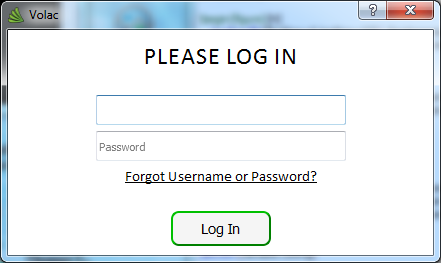
\includegraphics[width=\textwidth]{./Maintenance/Images/LoginWindow.png}
    \caption{The login screen that is displayed on initial startup.} \label{fig:LoginWindow}
\end{figure}

\begin{figure}[H]
    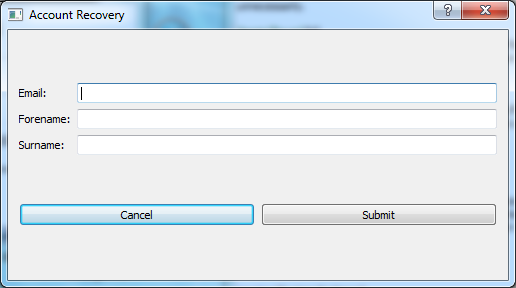
\includegraphics[width=\textwidth]{./Maintenance/Images/AccountRecovery.png}
    \caption{Account recovery window if the "forgotten username or password" button is clicked} \label{fig:AccountRecovery}
\end{figure}

\begin{figure}[H]
    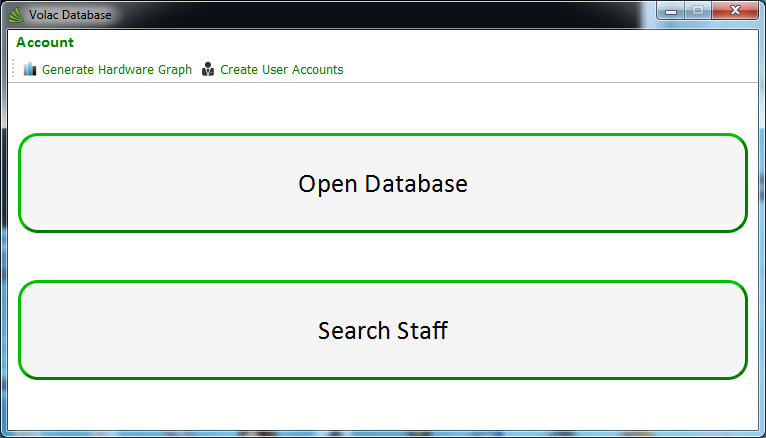
\includegraphics[width=\textwidth]{./Maintenance/Images/adminmainmenu.png}
    \caption{Admin main menu interface after log in} \label{fig:adminmainmenu}
\end{figure}

\begin{figure}[H]
    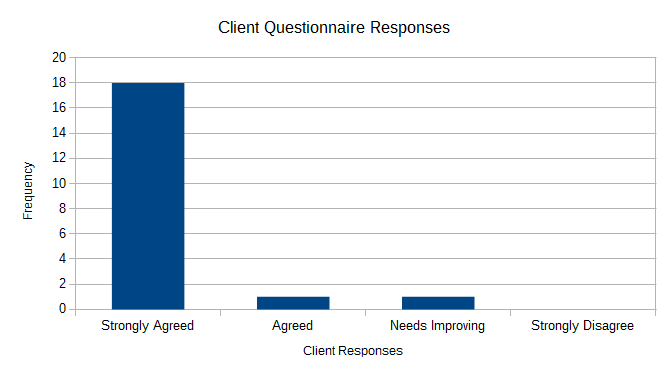
\includegraphics[width=\textwidth]{./Maintenance/Images/graph.png}
    \caption{Graph output showing departments number of hardware devices, activated when toolbar button is clicked} \label{fig:graph}
\end{figure}

\begin{figure}[H]
    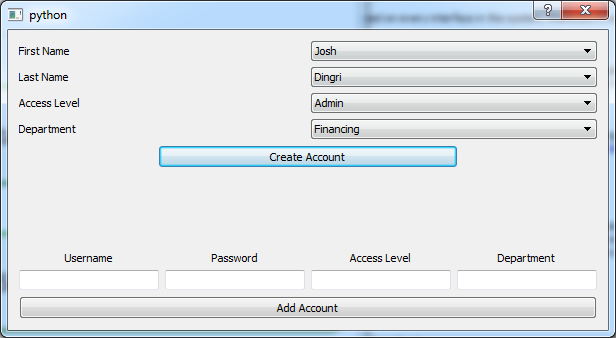
\includegraphics[width=\textwidth]{./Maintenance/Images/createaccounts.png}
    \caption{Create accounts window activated when toolbar button is clicked} \label{fig:createaccounts}
\end{figure}

\begin{figure}[H]
    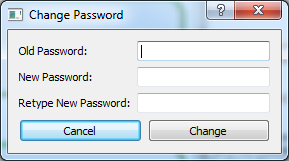
\includegraphics[width=\textwidth]{./Maintenance/Images/changepassword.png}
    \caption{Change password window activated when toolbar button is clicked} \label{fig:changepassword}
\end{figure}

\begin{figure}[H]
    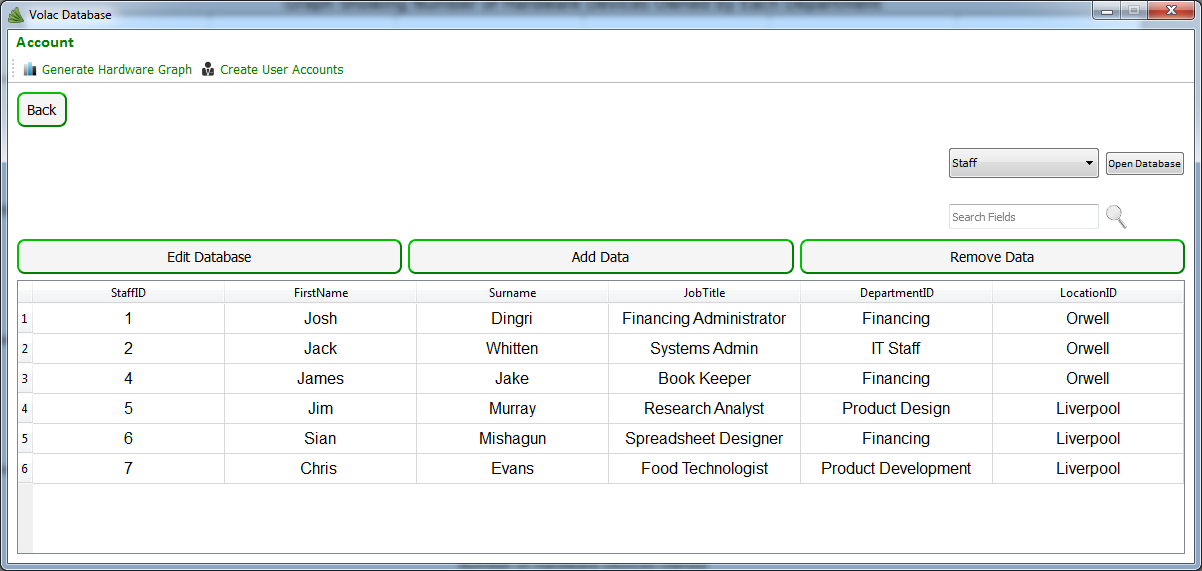
\includegraphics[width=\textwidth]{./Maintenance/Images/opendb.png}
    \caption{Open database interface, shown when user clicks button on the main menu} \label{fig:opendb}
\end{figure}

\begin{figure}[H]
    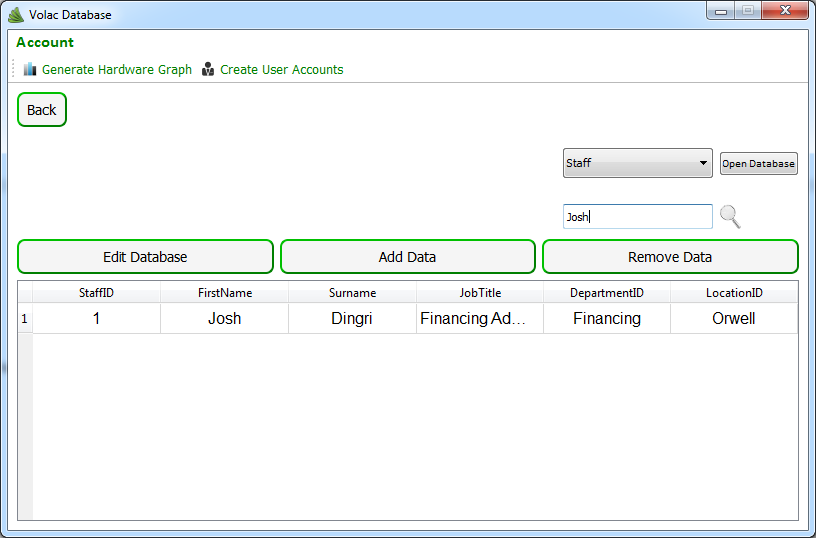
\includegraphics[width=\textwidth]{./Maintenance/Images/Searched.png}
    \caption{Result after text is entered into the search box} \label{fig:Searched}
\end{figure}

\begin{figure}[H]
    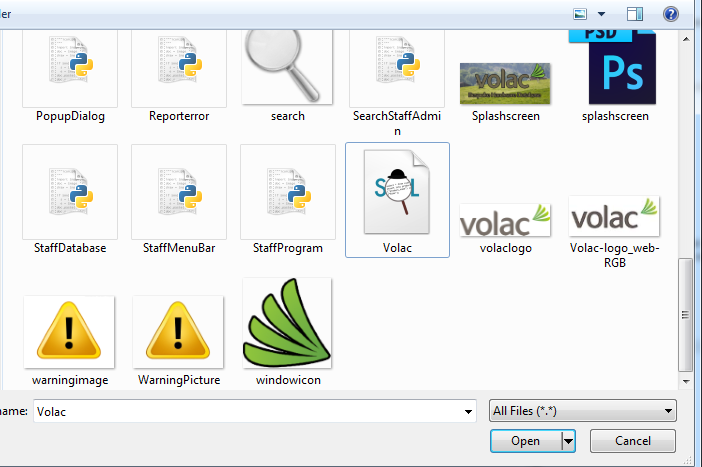
\includegraphics[width=\textwidth]{./Maintenance/Images/filebrowser.png}
    \caption{File browser to allow the user to choose the database file} \label{fig:filebrowser}
\end{figure}

\begin{figure}[H]
    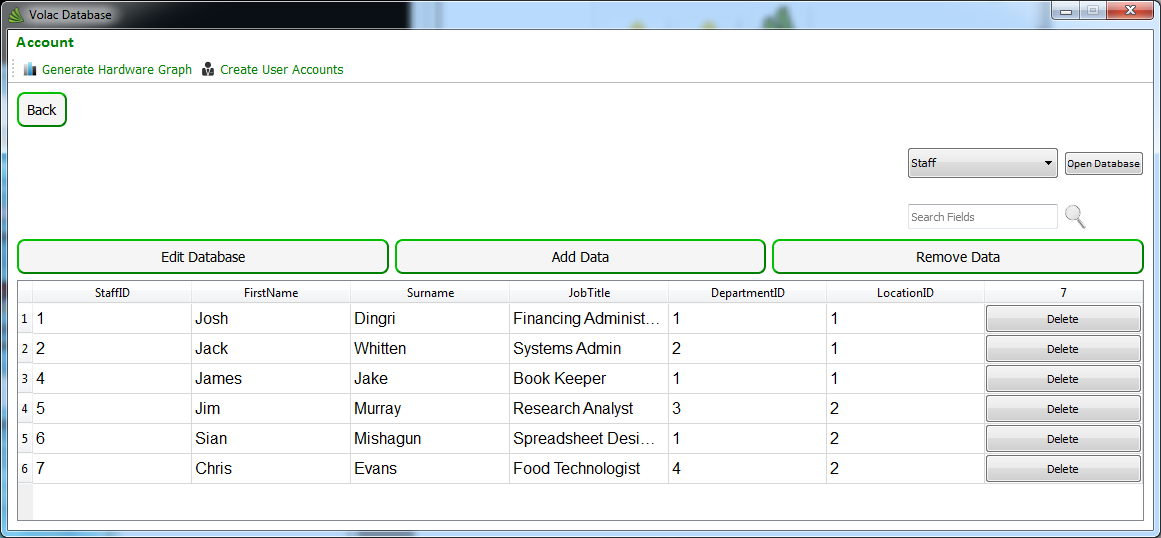
\includegraphics[width=\textwidth]{./Maintenance/Images/deletingdata.png}
    \caption{Delete buttons shown when the remove data button is pressed} \label{fig:deletingdata}
\end{figure}

\begin{figure}[H]
    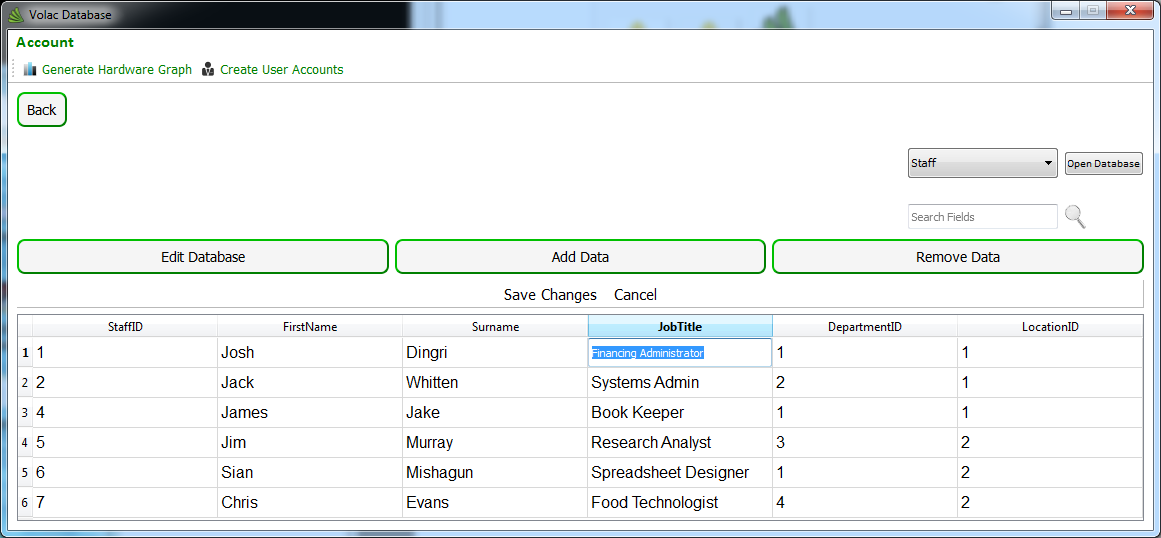
\includegraphics[width=\textwidth]{./Maintenance/Images/EditingData.png}
    \caption{User can edit data when edit data button is pressed} \label{fig:EditingData}
\end{figure}

\begin{figure}[H]
    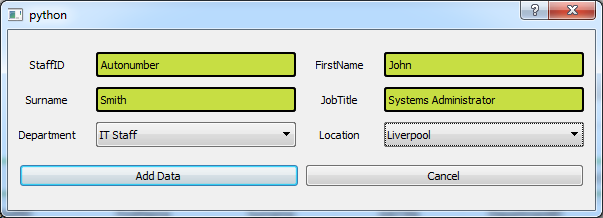
\includegraphics[width=\textwidth]{./Maintenance/Images/AddingData.png}
    \caption{The add data window to add data to the database.} \label{fig:AddingData}
\end{figure}

\begin{figure}[H]
    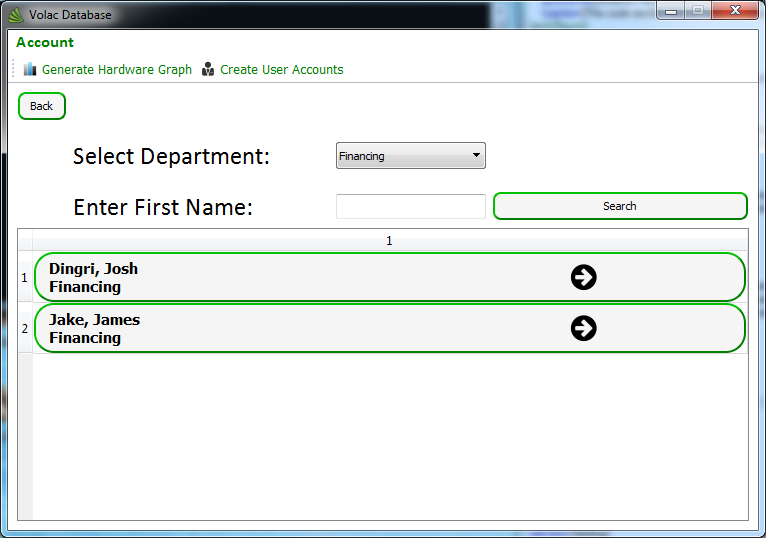
\includegraphics[width=\textwidth]{./Maintenance/Images/searchstaff.png}
    \caption{Search staff interface to search staff by department} \label{fig:searchstaff}
\end{figure}

\begin{figure}[H]
    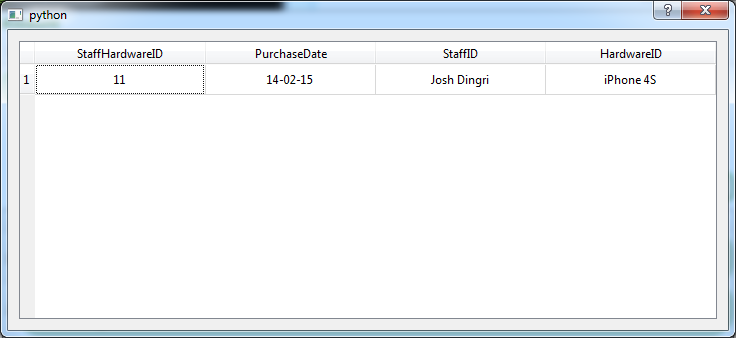
\includegraphics[width=\textwidth]{./Maintenance/Images/searchstaffresult.png}
    \caption{Window showing more information when a staff member is clicked on the search staff screen} \label{fig:searchstaffresult}
\end{figure}

\begin{figure}[H]
    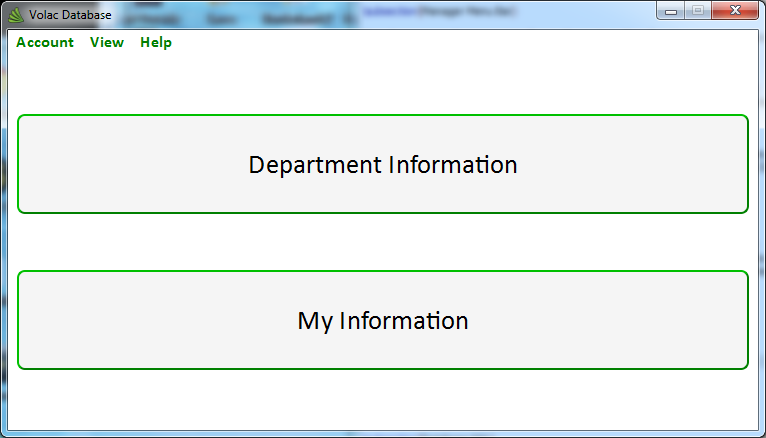
\includegraphics[width=\textwidth]{./Maintenance/Images/ManagerMM.png}
    \caption{Manager main menu after log in} \label{fig:ManagerMM}
\end{figure}

\begin{figure}[H]
    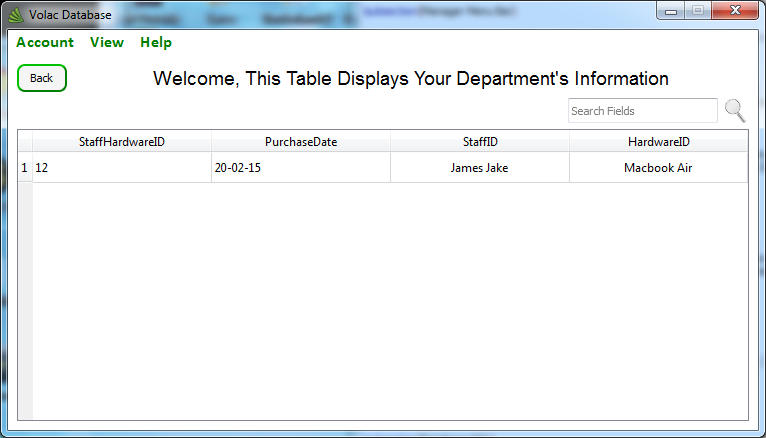
\includegraphics[width=\textwidth]{./Maintenance/Images/departinfo.png}
    \caption{Department information on manager interface} \label{fig:departinfo}
\end{figure}

\begin{figure}[H]
    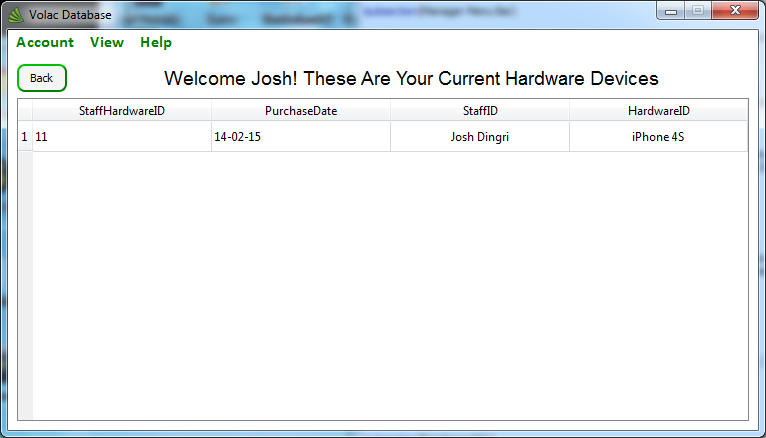
\includegraphics[width=\textwidth]{./Maintenance/Images/myinfomanager.png}
    \caption{Personal information ("My Information") interface shown for managers} \label{fig:myinfomanager}
\end{figure}

\begin{figure}[H]
    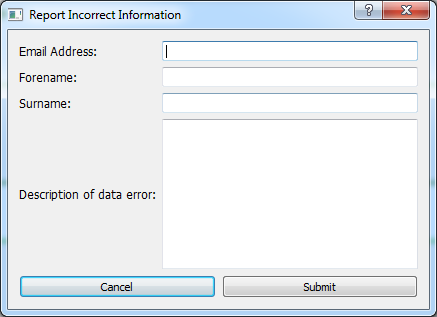
\includegraphics[width=\textwidth]{./Maintenance/Images/ReportError.png}
    \caption{The report errors email interface after toolbar button click} \label{fig:ReportError}
\end{figure}

\begin{figure}[H]
    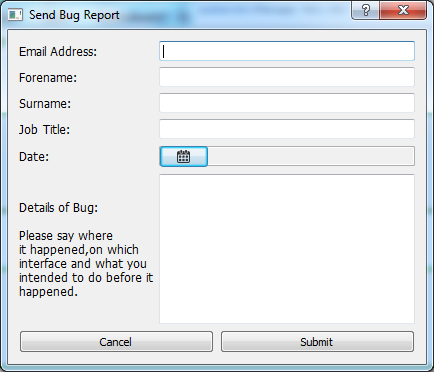
\includegraphics[width=\textwidth]{./Maintenance/Images/ReportBug.png}
    \caption{The report bug email interface after toolbar button click} \label{fig:ReportBug}
\end{figure}

\begin{figure}[H]
    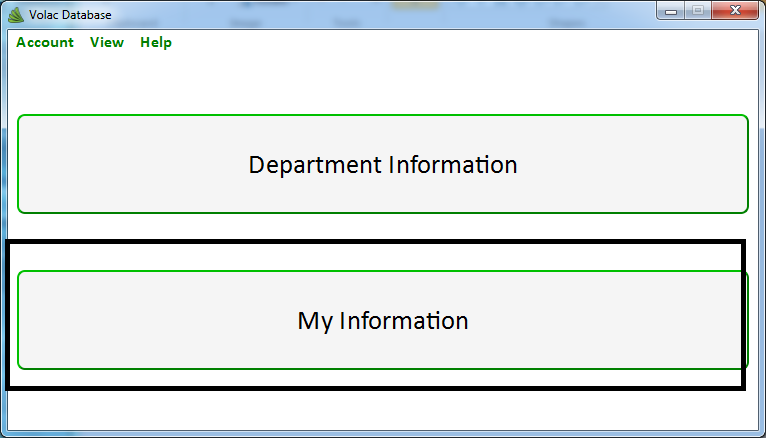
\includegraphics[width=\textwidth]{./Maintenance/Images/myinfo.png}
    \caption{Staff interface after login also showing personal information ("My Information") for staff} \label{fig:myinfo}
\end{figure}




\subsection{ER Diagram}

\begin{figure}[H]
    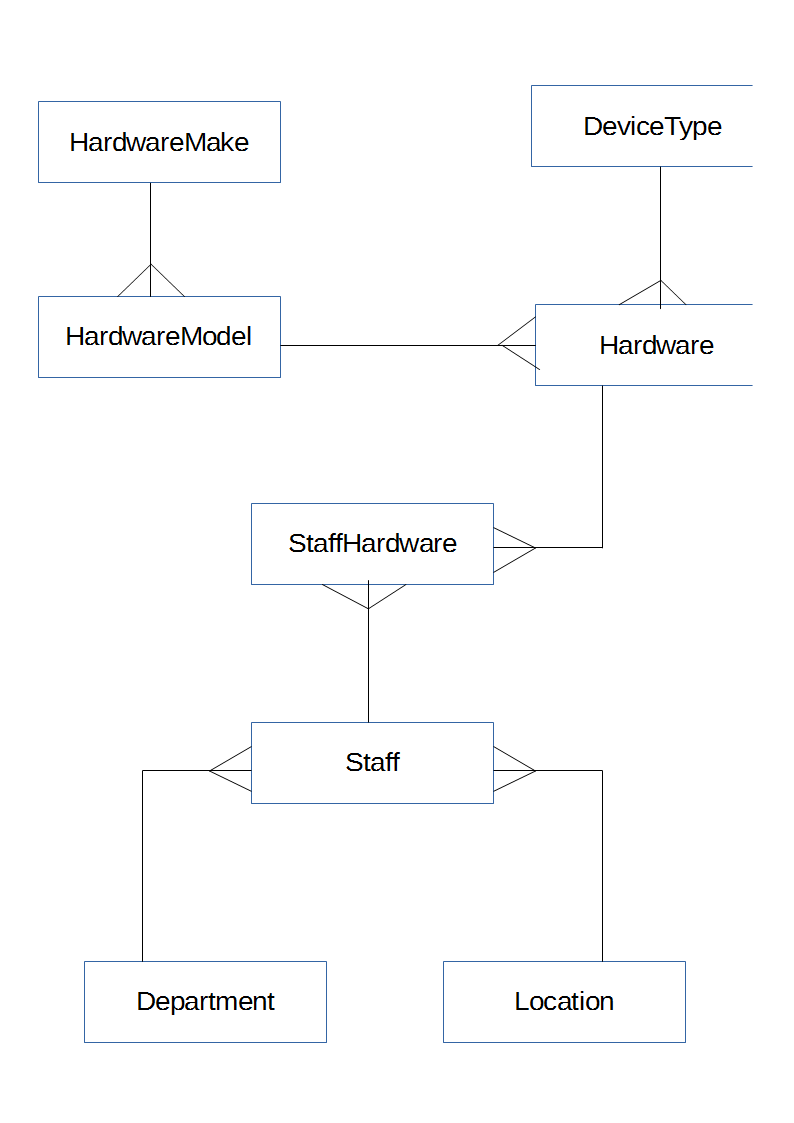
\includegraphics[width=\textwidth]{./Maintenance/Images/erupdateddiagram.png}
    \caption{Above is my final database which has been displayed as an Entity Relationship Diagram. It has changed slightly since my initial design.} \label{fig:erdiagram}
\end{figure}

\subsection{Database Table Views}

\begin{figure}[H]
    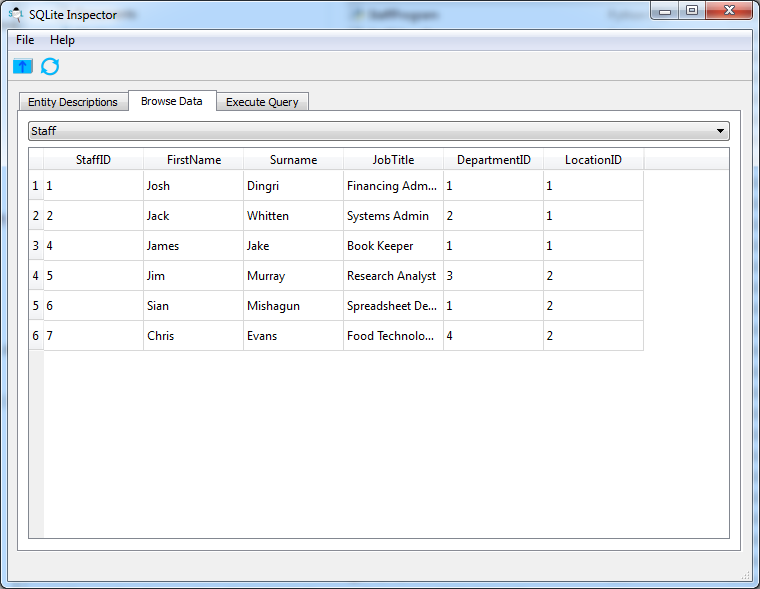
\includegraphics[width=\textwidth]{./Maintenance/Images/StaffTable.png}
    \caption{The "'Staff"' entity has 6 fields. The primary key of this entity is "StaffID". "DepartmentID" is a forein key that links to the "Department" entity (Fig: \ref{fig:DepartmentTable}) . "LocationID" is also a foreign key that links to the "Location" entity. (Fig: \ref{fig:LocationTable})} \label{fig:StaffTable}
\end{figure}

\begin{figure}[H]
    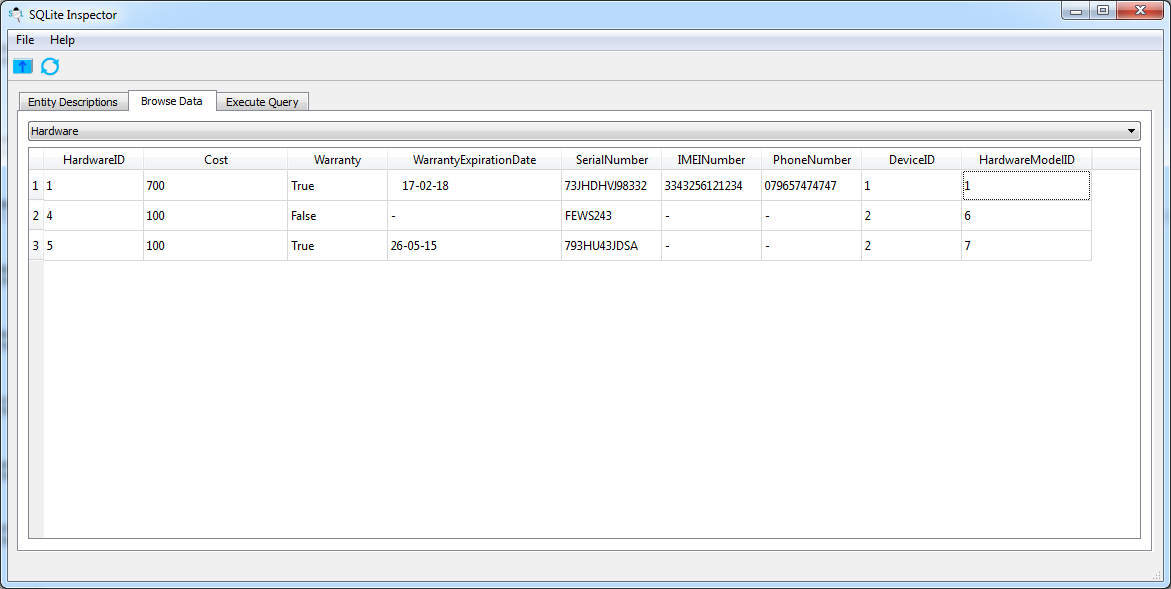
\includegraphics[width=\textwidth]{./Maintenance/Images/HardwareTable.png}
    \caption{The"Hardware" entity has 9 fields. The primary key of this entity is "HardwareID". "DeviceID" is a foreign key that links to the "DeviceType" entity  (Fig: \ref{fig:DeviceType}). "HardwareModelID" is also a foreign key that links to the "HardwareModel" entity (Fig: \ref{fig:HardwareModelTable})} \label{fig:HardwareTable}
\end{figure}

\begin{figure}[H]
    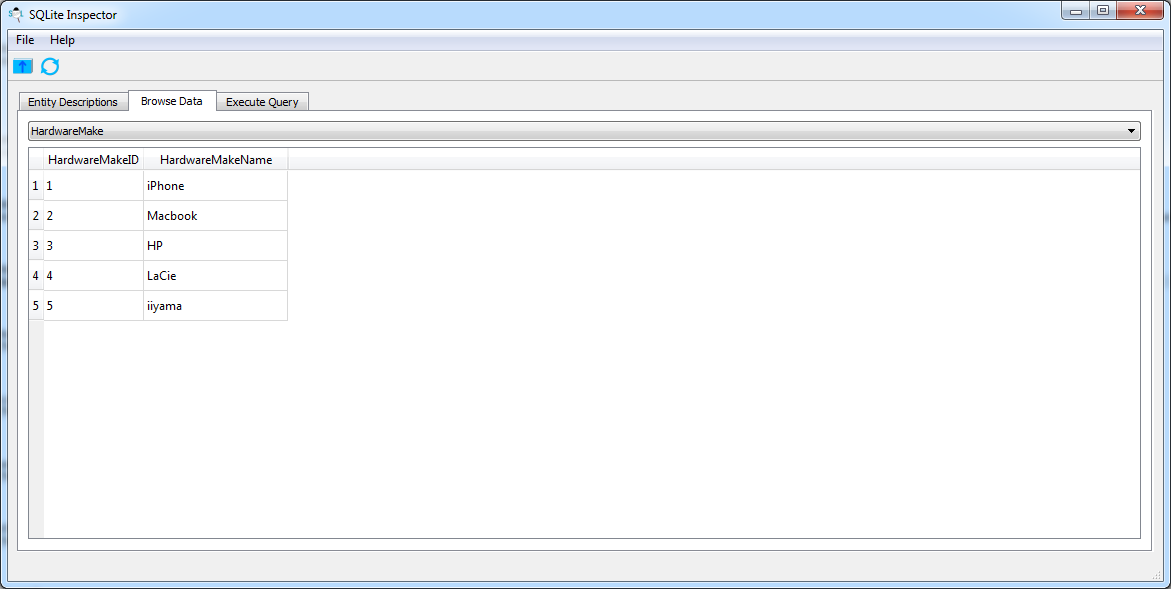
\includegraphics[width=\textwidth]{./Maintenance/Images/HardwareMakeTable.png}
    \caption{The "HardwareMake" entity has 2 fields. The primary key is "HardwareMakeID". The only store of data is the "HardwareMakeName" field} \label{fig:HardwareMakeTable}
\end{figure}

\begin{figure}[H]
    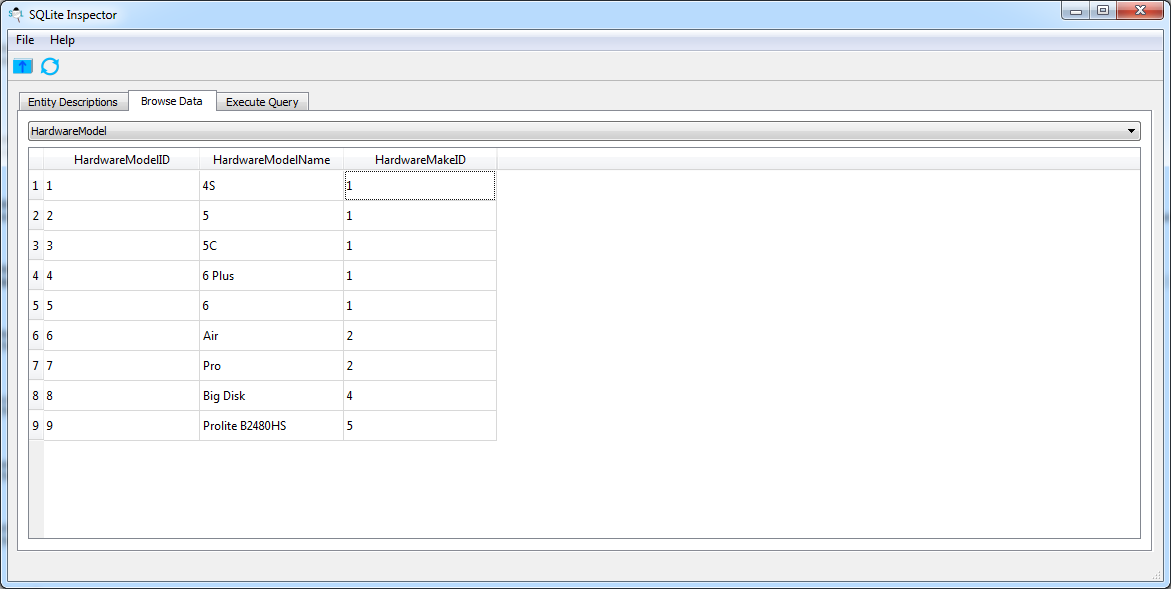
\includegraphics[width=\textwidth]{./Maintenance/Images/HardwareModelTable.png}
    \caption{The "HardwareModel" entity has 3 fields. The primary key is "HardwareModelID". The foreign key in this entity is "HardwareMakeID" which links to the "HardwareMake" entity. (Fig: \ref{fig:HardwareMakeTable})} \label{fig:HardwareModelTable}
\end{figure}

\begin{figure}[H]
    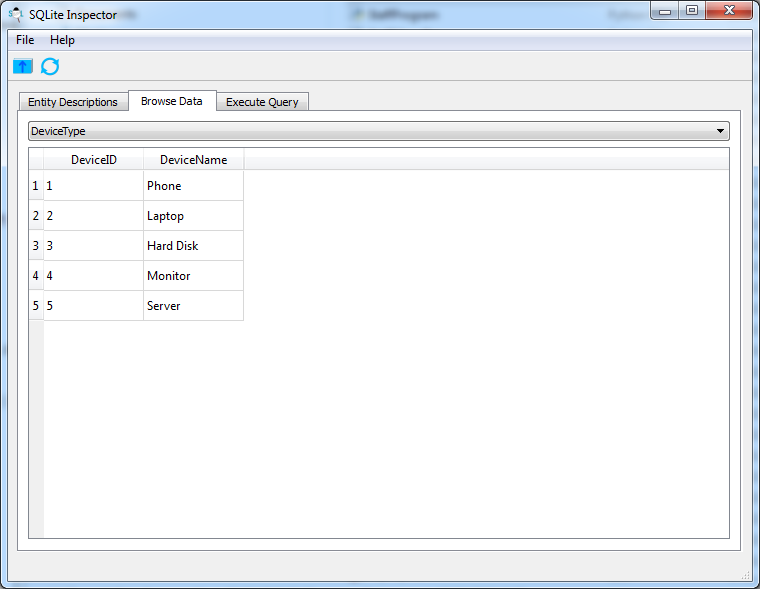
\includegraphics[width=\textwidth]{./Maintenance/Images/DeviceType.png}
    \caption{The "DeviceType" entity has 2 fields. The primary key is "DeviceID". The only store of data is the "DeviceName" field} \label{fig:DeviceType}
\end{figure}

\begin{figure}[H]
    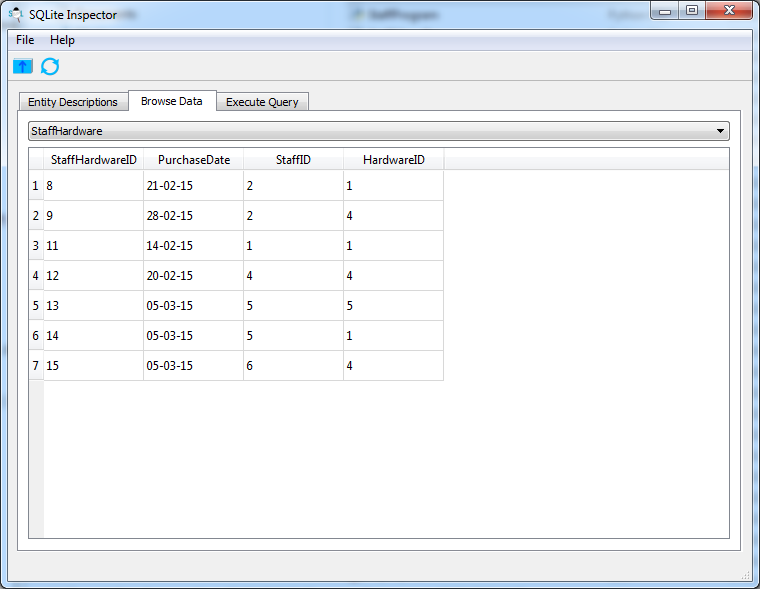
\includegraphics[width=\textwidth]{./Maintenance/Images/StaffHardware.png}
    \caption{The"StaffHardware" entity has 4 fields. The primary key of this entity is "StaffHardwareID". "StaffID" is a foreign key that links to the "Staff" entity  (Fig: \ref{fig:StaffTable}). "HardwareID" is also a foreign key that links to the "Hardware" entity (Fig: \ref{fig:HardwareTable})} \label{fig:StaffHardware}
\end{figure}

\begin{figure}[H]
    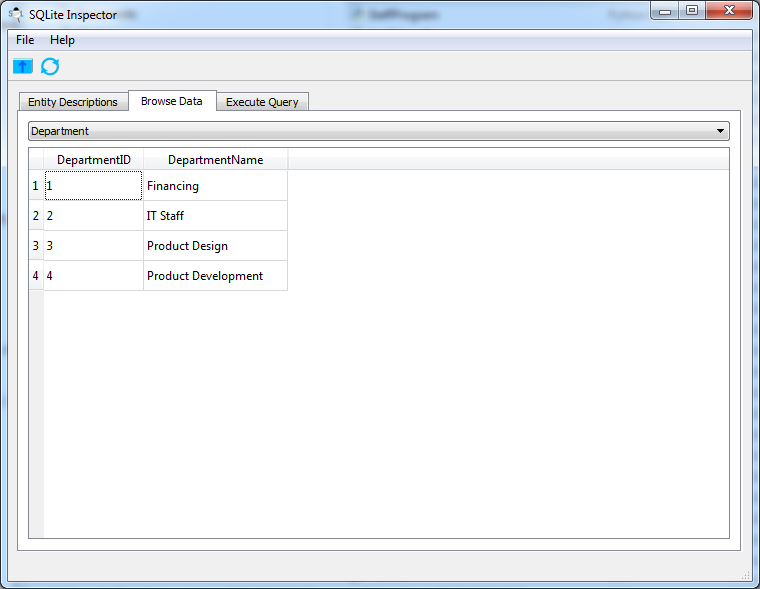
\includegraphics[width=\textwidth]{./Maintenance/Images/DepartmentTable.png}
    \caption{The "Department" entity has 2 fields. The primary key is "DepartmentID". The only store of data is the "DepartmentName" field} \label{fig:DepartmentTable}
\end{figure}

\begin{figure}[H]
    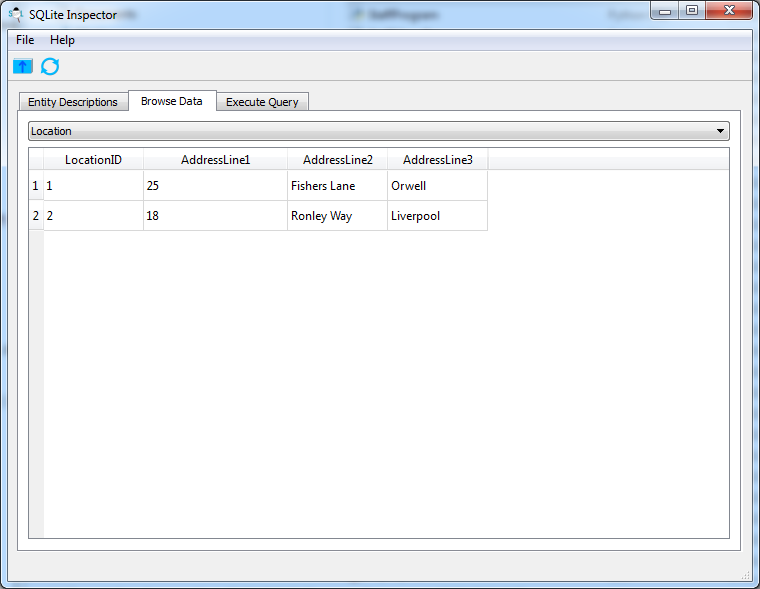
\includegraphics[width=\textwidth]{./Maintenance/Images/LocationTable.png}
    \caption{The "Location" entity has 4 fields. The primary key is "LocationID". The entity stores location details in the other 3 fields} \label{fig:LocationTable}
\end{figure}

\begin{figure}[H]
    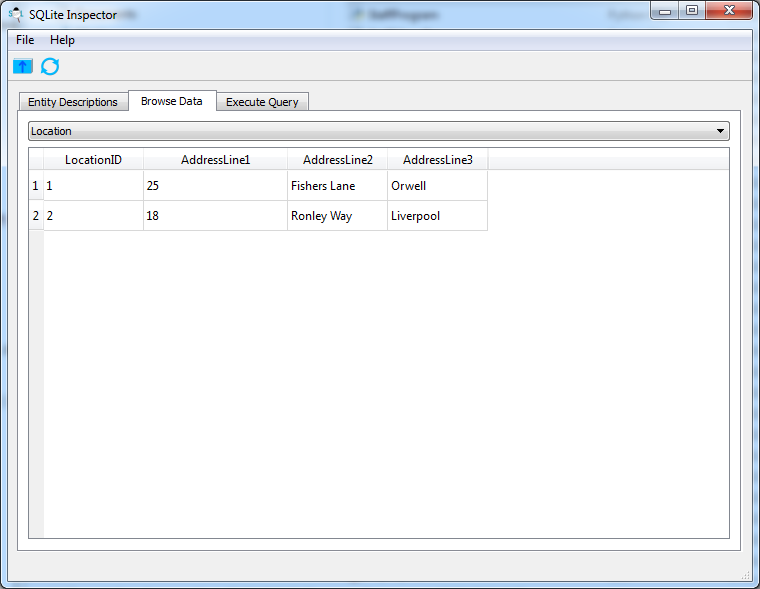
\includegraphics[width=\textwidth]{./Maintenance/Images/LocationTable.png}
    \caption{The "Location" entity has 4 fields. The primary key is "LocationID". The entity stores location details in the other 3 fields} \label{fig:LocationTable}
\end{figure}

The below database has only one table in it and its purpose is to store usernames and passwords as well as other details including access rights. This is not part of the relational database, although looking back it should have been another table in the original instead of a new one.

\begin{figure}[H]
    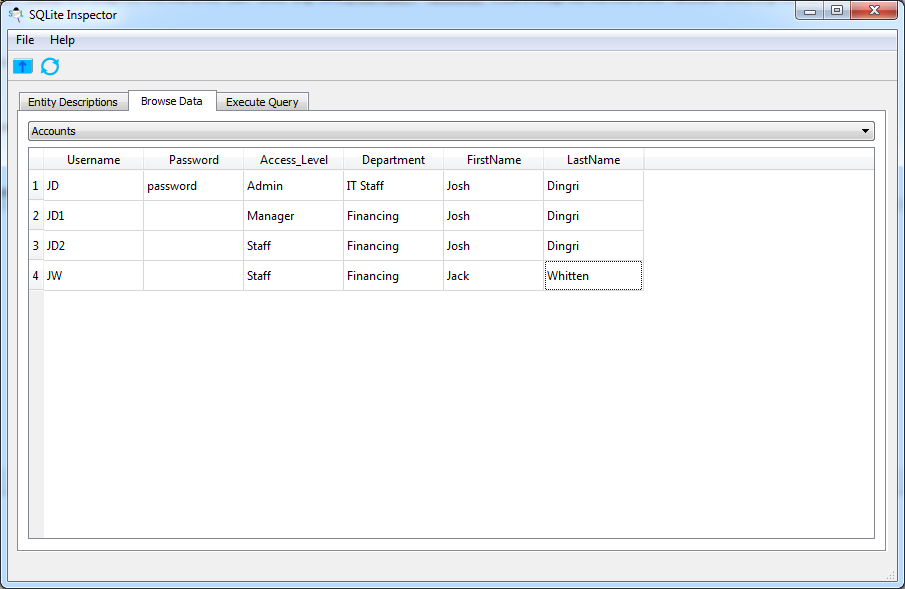
\includegraphics[width=\textwidth]{./Maintenance/Images/accountsdb.png}
    \caption{The primary key is the username} \label{fig:accountstable}
\end{figure}

\subsection{Database SQL}

The below is the SQL code which created each entity in the database.

\subsubsection{Staff Entity}

 \pythonfile[firstline=26,lastline=38]{./Implementation/Files/StaffDatabase.py}

\subsubsection{Hardware Entity}

 \pythonfile[firstline=40,lastline=55]{./Implementation/Files/StaffDatabase.py}

\subsubsection{HardwareMake Entity}

 \pythonfile[firstline=57,lastline=62]{./Implementation/Files/StaffDatabase.py}

\subsubsection{HardwareModel Entity}

 \pythonfile[firstline=64,lastline=72]{./Implementation/Files/StaffDatabase.py}

\subsubsection{DeviceType Entity}

 \pythonfile[firstline=74,lastline=79]{./Implementation/Files/StaffDatabase.py}

\subsubsection{StaffHardware Entity}

 \pythonfile[firstline=81,lastline=90]{./Implementation/Files/StaffDatabase.py}

\subsubsection{Department Entity}

 \pythonfile[firstline=92,lastline=97]{./Implementation/Files/StaffDatabase.py}

\subsubsection{Location Entity}

 \pythonfile[firstline=99,lastline=106]{./Implementation/Files/StaffDatabase.py}

\subsubsection{Creation of all the tables}

 \pythonfile[firstline=3,lastline=24]{./Implementation/Files/StaffDatabase.py}

\subsubsection{Creation of accounts table}

 \pythonfile[firstline=1]{./Implementation/Files/Logins.py}

\subsection{SQL Queries}

\begin{center}
    \begin{longtable}{|p{3cm}|p{7cm}|p{2cm}|}
    \hline
	\textbf{Functionality/ Description} & \textbf{SQL Query} & \textbf{Reference} \\ \hline

Retreives all fields for one user & \sqlinline{SELECT * FROM Accounts WHERE Username=?} & Full Code: \ref{LW} Page: \pageref{LW} \\ \hline
Retrieves all fields for specified table &  \sqlinline{"SELECT * FROM \{\}".format(CurrentCBValue)}& Full Code: \ref{ADGUI} Page: \pageref{ADGUI} \\ \hline
Retrieves all department names from database &  \sqlinline{SELECT DepartmentName FROM Department}& Full Code: \ref{ADGUI} Page: \pageref{ADGUI} \\ \hline
Retrieves all address line 3 fields from database &  \sqlinline{SELECT AddressLine3 FROM Location}& Full Code: \ref{ADGUI} Page: \pageref{ADGUI} \\ \hline
Retrieves all hardware make name fields  from database &  \sqlinline{SELECT HardwareMakeName FROM HardwareMake}& Full Code: \ref{ADGUI} Page: \pageref{ADGUI} \\ \hline
Retrieves First Name and Surname from database &  \sqlinline{SELECT FirstName,Surname FROM Staff}& Full Code: \ref{ADGUI} Page: \pageref{ADGUI}  \\ \hline
Retrieves all HardwareMakeName fields from database &  \sqlinline{SELECT HardwareMakeName FROM HardwareMake}& Full Code: \ref{ADGUI} Page: \pageref{ADGUI}   \\ \hline
Retrieves all HardwareMakeIDs that have the specified HardwareModelID &  \sqlinline{SELECT HardwareMakeID FROM HardwareModel WHERE HardwareModelID IN \{\}".format(self.hardwaremodelid)}& Full Code: \ref{ADGUI} Page: \pageref{ADGUI}  \\ \hline
Retrieves all HardwareMakeNames that have specified HardwareMakeIDs & \sqlinline{SELECT HardwareMakeName FROM HardwareMake WHERE HardwareMakeID IN \{\}".format(self.MakeID)}& Full Code: \ref{ADGUI} Page: \pageref{ADGUI} \\ \hline
Retrieves all Device Names from database & \sqlinline{SELECT DeviceName FROM DeviceType}& Full Code: \ref{ADGUI} Page: \pageref{ADGUI} \\ \hline
Retrieves a DepartmentID & \sqlinline{SELECT DepartmentID FROM Department WHERE DepartmentName=?",(text,)}& Full Code: \ref{ADGUI} Page: \pageref{ADGUI} \\ \hline
Retrieves a LocationID & \sqlinline{SELECT LocationID FROM Location WHERE AddressLine3=?",(text,)}& Full Code: \ref{ADGUI} Page: \pageref{ADGUI} \\ \hline
Retrieves a HardwareModelID &\sqlinline{SELECT HardwareModelID FROM HardwareModel WHERE HardwareModelName=?",(text,)}& Full Code: \ref{ADGUI} Page: \pageref{ADGUI} \\ \hline
Retrieves a HardwareMakeID & \sqlinline{SELECT HardwareMakeID FROM HardwareMake WHERE HardwareMakeName=?",(text,)}& Full Code: \ref{ADGUI} Page: \pageref{ADGUI} \\ \hline
Retrieves a StaffID & \sqlinline{SELECT StaffID FROM Staff WHERE Surname =? AND FirstName =?",(split[1],split[0],)}&Full Code: \ref{ADGUI} Page: \pageref{ADGUI}  \\ \hline
Retrieves a HardwareMakeID & \sqlinline{SELECT HardwareMakeID FROM HardwareMake WHERE HardwareMakeName =?",(text,)}&Full Code: \ref{ADGUI} Page: \pageref{ADGUI}  \\ \hline
Retrieves a HardwareModelName & \sqlinline{SELECT HardwareModelName FROM HardwareModel WHERE HardwareMakeID=?",(HardwareID[0],)}&Full Code: \ref{ADGUI} Page: \pageref{ADGUI}  \\ \hline
Retrieves a HardwareModelID from database & \sqlinline{SELECT HardwareModelID FROM Hardware}& Full Code: \ref{ADGUI} Page: \pageref{ADGUI} \\ \hline
Retrieves a HardwareModelName & \sqlinline{SELECT HardwareModelName FROM HardwareModel WHERE HardwareMakeID = '\{\}' AND HardwareModelID IN \{\}".format(HardwareMakeID[0], HardwareModels)}& Full Code: \ref{ADGUI} Page: \pageref{ADGUI} \\ \hline
Retrieves a HardwareModelID & \sqlinline{SELECT HardwareModel.HardwareModelID FROM HardwareMake,HardwareModel WHERE HardwareMake.HardwareMakeName =? AND HardwareModel.HardwareModelName =?",(MakeName,ModelName,)}&Full Code: \ref{ADGUI} Page: \pageref{ADGUI} \\ \hline
Retrieves a HardwareMakeID & \sqlinline{SELECT HardwareModel.HardwareMakeID, HardwareModel .HardwareModelID FROM HardwareModel,HardwareMake WHERE HardwareMake.HardwareMakeName =? AND HardwareModelName =?",(MakeName,ModelName,)}&Full Code: \ref{ADGUI} Page: \pageref{ADGUI} \\ \hline
Retrieves a HardwareMakeID & \sqlinline{SELECT Hardware.HardwareID FROM Hardware,HardwareModel WHERE Hardware.HardwareModelID =? AND HardwareModel.HardwareMakeID=?" , (HardwareModelIDs[1], HardwareModelIDs[0],)}&Full Code: \ref{ADGUI} Page: \pageref{ADGUI}  \\ \hline
Retrieves a DeviceID & \sqlinline{SELECT DeviceID FROM DeviceType WHERE DeviceName=?",(text,)}&Full Code: \ref{ADGUI} Page: \pageref{ADGUI} \\ \hline
Retrieves all HardwareID fields with the specified WarrantyExpirationDate & \sqlinline{SELECT HardwareID FROM Hardware WHERE WarrantyExpirationDate=?", (self.purchasedate,)}& Full Code: \ref{MP} Page: \pageref{MP}\\ \hline
Retrieves a list of all the table names in the database &  \sqlinline{SELECT name FROM sqlite\_master WHERE type = 'table';}& Full Code: \ref{MP} Page: \pageref{MP}\\ \hline


Inserts data (values) into fields (self.col) & \sqlinline{insert into \{0\} values \{1\}".format(self.col,values)}& Full Code: \ref{ADGUI} Page: \pageref{ADGUI}\\ \hline
Inserts the placeholder values into the Accounts table with the fields shown & \sqlinline{insert into Accounts(Username, Password, Access_Level, Department, FirstName,LastName) values (?,?,?,?,?,?)}& Full Code: \ref{AAI} Page: \pageref{AAI} \\ \hline
Overwrites original password with new password for the specified user &  \sqlinline{UPDATE Accounts SET Password=? WHERE Username=?",(new_password, self.username,)}&  Full Code: \ref{CP} Page: \pageref{CP} \\ \hline
Statement is ran when a cell value is changed and will update original text with current text entered & \sqlinline{update \{0\} set \{1\} where \{2\}=\{3\}".format(self.currentcbvalue, self.Columnname, self.ID, self.IDtoChange)}&  Full Code: \ref{ODW} Page: \pageref{ODW} \\ \hline

Statement ran when delete button is clicked, it will delete the whole record that the button was in & \sqlinline{delete from \{0\} where \{1\}=\{2\}".format(self.currentcbvalue, self.ID, self.IDtoChange)}& Full Code: \ref{ODW} Page: \pageref{ODW}  \\ \hline

\end{longtable}
\end{center}

\section{Testing}

\subsection{Summary of Results}

Testing largely proved that my system was reliable and robust as there were only a few errors that were found with the system. Overall the system meets most of the original objectives and when implementing these objectives I made sure I started with the most desired first. All of the necessary objectives have been met however the additional objectives the client would have liked to have, for example having an on line database, have been left out which was mainly due to lack of time. There have also been quite a few additional features that were implemented that will benefit the user in different ways such as the generation of graphs. The additional features along with the full testing table can be found at 3.1.4 on page 179.

\subsection{Known Issues}

There is only a couple of known issues with my current code. When viewing the database tables in any interface the foreign keys are presented as text and are user friendly like the client requested. However if the user clicks the "Edit Data" button (\ref{fig:EditingData}) or "Remove Data" button (\ref{fig:deletingdata}) the foreign keys will switch back to integers which make it hard for the user to understand what is going on. This can be fixed with drop down boxes at a later date. Another problem that I will need to fix is the fact that in order for the automatic warranty expiration email to send the program will need to be restarted every day. This is obviously not ideal since the client may want to leave the system running on a server at some point. It also means every time the system is reopened 90 days before expiration of an item they will get an email. Validation when editing data does not currently work, this is not a huge issue since the data would have already been validated during input, the fix for this issue should be fairly straight forward as it just relies on copying the same validation from the input screen.

\section{Code Explanations}

\subsection{Difficult Sections}

\subsubsection{Adding Data}

The method of adding data may be complicated to understand to a programmer viewing my code. I have added comments to aid anyone who is maintaining the code.

The overall idea behind the module is to get the current table that is selected from the  "Open Database" interface and find the headings for that table. The program will then use these headings as the labels for the GUI, the line edits are generated by adding a space after every label which are later converted into line edits. This approach was perfect in the short term but as I was adding validation and combo boxes the generic method no longer worked as intended as specific validations needed to be given to line edits. This is why there are boolean statements so if a certain label exists a validation function can be ran.

The full section that I will be annotating can be found here: \ref{ADGUI} on page \pageref{ADGUI}
\begin{landscape}

\begin{figure}[H]
    \pythonfile[firstline=25,lastline=36]{./Implementation/Files/AddDataGui.py}
    \caption{The purpose of this part of the module is to first get the column headings (self.col) and then create a grid layout with the exact number of spaces to store the labels and line edits (positions). The position variable basically divides the number of columns in half as there will always be two columns of labels. It is rounded if its an odd number and +1 is added in case the odd number needs the extra row at the bottom. The range of 4 is added so there can be 4 columns (2 columns of labels and line edits) \newline The self.col variable will add a space in between each label (later to be replaced by a line edit)}  
\end{figure}

\begin{figure}[H]
    \pythonfile[firstline=66,lastline=76]{./Implementation/Files/AddDataGui.py}
    \caption{The for loop with the Zip function allows iteration over two loops a the same time. The self.col and positions are renamed and instead, inside the for loop, they are referenced as name and position. \newline The IF statement will run and replace all the spaces with line edits.}  
\end{figure}

\begin{figure}[H]
    \pythonfile[firstline=346,lastline=362]{./Implementation/Files/AddDataGui.py}
    \caption{The IF statements shown above will look for the label which is stated. They will then apply a validation to them which is why a boolean value is stated. The boolean statements will run another IF statement to allows the line edit connected to the label to be validated (shown below)}  
\end{figure}

\pythonfile[firstline=334,lastline=341]{./Implementation/Files/AddDataGui.py}

\begin{figure}[H]
    \pythonfile[firstline=435,lastline=442]{./Implementation/Files/AddDataGui.py}
    \caption{When a identifier is used as a label the program will strip the last 2 letters off the end making it more user friendly. For example HardwareMakeID becomes HardwareMake}  
\end{figure}


\subsubsection{Foreign Key Management and Table Structure}

Since I have used QTableWidget for my tables in the system, I had a different method of refrencing foreigns keys using text  than models with QTableView. Because of this it may be quite difficult for a programmer to understand how it works.

The full section that I will be annotating can be found here: \ref{ODW} on page \pageref{ODW}

\begin{figure}[H]
    \pythonfile[firstline=195,lastline=198]{./Implementation/Files/OpenDatabaseWindow.py}
    \caption{This section adds data to the table, all foreign keys at this point are integer values.}  
\end{figure}

\begin{figure}[H]
\begin{small}
    \pythonfile[firstline=200,lastline=215]{./Implementation/Files/OpenDatabaseWindow.py}
\end{small}
    \caption{To created user friendly foreign keys I have hard coded in the different headers that require foreign keys (eg. DepartmentID, LocationID, DeviceID). The code section above will look at if the current header is "DepartmentID" and if it is the correct foreign key value will be displayed based on the integer value of the cell (see above section).\newline Line 7 will take the integer value and convert it into a text value. This is where the text based foreign keys created.}  
\end{figure}

\begin{figure}[H]
\begin{small}
    \pythonfile[firstline=216,lastline=229]{./Implementation/Files/OpenDatabaseWindow.py}
\end{small}
    \caption{This is another example showing a different column heading. On line 5 it will take the LocationID (integer value) and find the Location (text value) and add it to the table on line 12.}  
\end{figure}

The sections are repeated for every column header. Although this method works, it is not very efficient. This problem exists because I initially started to use QTableWidget not QTableView. Using QTableView would have been much easier and more efficient since I could have used sql models to view foreign keys more efficiently.
\newpage
\subsubsection{Changing Passwords}

The code for this section may be confusing as it references the database table quite a lot with indexing. Therefore it is important to explain how this works. This module is used for all interfaces to change their current password (for logging into the system) and is activated through the menubar.

Full code can be found here: \ref{CP} on page \pageref{CP}

\begin{figure}[H]
    \pythonfile[firstline=63,lastline=83]{./Implementation/Files/ChangePassword.py}
    \caption{This method (part of the "ChangePassword" class) is ran in order to get the text input from the change password GUI and use these details to change the user's password.\newline Line 5 gets the username from the database for the specific user, the variable (new\_password) is then referenced on line 11. \newline Line 7 references the password field in the database table for the specific user. It will check if the old password entered into the line edit matches the password in the database. \newline Lines 15,18,21 change the label to visible, by default this label is hidden but is made visible again to display an error or confirmation of changed passwords.}  
\end{figure}


\subsection{Self-created Algorithms}

\subsubsection{Creating efficient and complex account details (Original (\ref{AAI})}

\begin{figure}[H]
    \pythonfile[firstline=124,lastline=143]{./Implementation/Files/AddingAccounts.py}
    \caption{This function works very well for task I set out to do. In my system it is necessary to create initial complex passwords and unique usernames that can then be emailed to staff. \newline The variable called "Username" combines the first letter of the first name with the surname and then adds a random digit between 1 and 100. This creates very good unique usernames automatically.\newline The "Password" variable creates a password 7 characters in length with random uppercase, lowercase letters and digits. This creates very secure passwords that staff can use until they manually change it.}  
\end{figure}


\subsubsection{Automatic Expiration Email (Original (\ref{MP})}

\begin{figure}[H]
    \pythonfile[firstline=121,lastline=132]{./Implementation/Files/MainProgram.py}
\end{figure}

\begin{figure}[H]
    \pythonfile[firstline=132,lastline=148]{./Implementation/Files/MainProgram.py}
    \caption{As the doc string states this function will check if a device has 90 days left before warranty ends. The function works well for what it does but it needs to be improved so it is only ran once a day and also ran when the program is left running. \newline WarrantyExpirationDate gets all dates from the database to check which ones are expiring. If the field has a '-' in, the field is ignored ('-' is added during input). \newline The variable 'currentdate' and 'self.WarrantyExpirationDate' shown on line 10 and 11 needed to be in the same format to be subtracted in the equation on line 15. The 'daysleft' variable will get the remaining days and if equal to 90 the email function will run. } 
\end{figure}

\subsubsection{Creating Graphs (Original (\ref{G})}

\begin{figure}[H]
    \pythonfile[firstline=11,lastline=33]{./Implementation/Files/Graph.py}
    \caption{The graph module will create a bar chart which will display how many hardware devices each department owns. Comments are also in place to help future programmers maintaining my program \newline 'NumberOfHardware' (line 8) will get all StaffIDs in the staffhardware table which will give the total amount of hardware devices. }  
\end{figure}

\begin{figure}[H]
    \pythonfile[firstline=39,lastline=49]{./Implementation/Files/Graph.py}
    \caption{The FOR loop along with list 'departmentnames' will display all the department names including duplications to count how many devices they own.}
\end{figure}

\begin{figure}[H]
    \pythonfile[firstline=51,lastline=68]{./Implementation/Files/Graph.py}
    \caption{The 'Counter' function will display how many devices each department owns in a dictionary format. \newline The dictionaries on line 14 are created dynamically and a dictionary is created for each department which is then added to the graph.}
\end{figure}

\end{landscape}
\section{Settings}

For distribution to my client I have compiled the Python files into an executable. The client can simply open this executable file to run the program therefore no additional settings need to be met.

However if someone was to continuing with the maintenance of my system they will need to install an extra module called 'matplotlib' that allows for the creation of graphs. When the client initially useds the system it would be sensible to create a new username/password from the one that is built in, they can then create there own secure log in details with sufficient privileges.   

\section{Acknowledgements}

\subsection{Calendar}

Code at \ref{C} on page \pageref{C}

Since I had never built a calendar before I did not know if it was a built in function or not. After browsing the Internet I found a calendar example on ZetCode which was the exact design I was looking for. 

\textbf{Link:} http://zetcode.com/gui/pyqt4/widgets/

\textbf{Original code}:

\begin{python}
#!/usr/bin/python
# -*- coding: utf-8 -*-

"""
ZetCode PyQt4 tutorial 

This example shows a QtGui.QCalendarWidget widget.

author: Jan Bodnar
website: zetcode.com 
last edited: September 2011
"""

import sys
from PyQt4 import QtGui, QtCore

class Example(QtGui.QWidget):
    
    def __init__(self):
        super(Example, self).__init__()
        
        self.initUI()
    
    
    def initUI(self):      

        cal = QtGui.QCalendarWidget(self)
        cal.setGridVisible(True)
        cal.move(20, 20)
        cal.clicked[QtCore.QDate].connect(self.showDate)
        
        self.lbl = QtGui.QLabel(self)
        date = cal.selectedDate()
        self.lbl.setText(date.toString())
        self.lbl.move(130, 260)
        
        self.setGeometry(300, 300, 350, 300)
        self.setWindowTitle('Calendar')
        self.show()
        
    def showDate(self, date):     
    
        self.lbl.setText(date.toString())
    
    
def main():
    
    app = QtGui.QApplication(sys.argv)
    ex = Example()
    sys.exit(app.exec_())


if __name__ == '__main__':
    main()
\end{python}

\subsection{Populating a QTableWidget}

Code at \ref{ODW} on page \pageref{ODW}

My program displayed tables using a QTableWidgets however I needed help learning how to populate these tables with data from my database. I came across a Stackoverflow answer explaining in detail the code needed to do this. It also included a function that was new to me called 'enumerate'. I researched and understood this function before I used the code otherwise it may have been confusing when it came to bug testing.

\textbf{Link:} http://stackoverflow.com/questions/11754825/inserting-data-from-sqlite-database-to-qtablewidget-using-pyqt-in-python

\textbf{Original Code:}

\begin{python}
cursor.execute('''SELECT * FROM MyTable''')
self.tblTable.setRowCount(cursor.rowcount)
for row, form in enumerate(cursor):
    for column, item in enumerate(form):
        self.tblTable.setItem(row, column, QtGui.QTableWidgetItem(str(item)))   
\end{python}

\subsection{Getting column names}

When I was producing my add data GUI it was necessary to use the database column names as labels for the line edits so the user knew what information to enter. I needed a way of extracting these column names into a list and using these names as labels. After searching the Internet I came across many Stackoverflow answers that showed the same kind of code. The specific answer I used is shown below.

Code at \ref{ADGUI} on page \pageref{ADGUI}

\textbf{Link:} http://stackoverflow.com/questions/9752372/how-do-i-get-the-column-names-from-a-row-returned-from-an-adodbapi-query

\textbf{Original Code:}

\begin{python}
col_names = [i[0] for i in cur.description]
\end{python}

\subsection{Positioning line edits on grid layout}

Before I started the Implementation I used a Zetcode code example to help create a calculator. One of the lines of code that I used was relevant for the task of positioning my line edits on a grid layout for the Add Data GUI. 
Code at \ref{ADGUI} on page \pageref{ADGUI}

\textbf{Link}: http://zetcode.com/gui/pyqt4/layoutmanagement/

\textbf{Original Code:}
\begin{python}
positions = [(i,j) for i in range(5) for j in range(4)]
\end{python}

\subsection{Regular Expressions}


Some of the regular expressions used in my system were researched on the Internet first in order to get the bet working design. Some of the results found have been directly taken from the sources.

\paragraph{Phone Number Regular Expression}
\
Code at \ref{ADGUI} on page \pageref{ADGUI}
\

 \textbf{Link}: http://stackoverflow.com/questions/3968049/regex-allow-a-string-to-only-contain-numbers-0-9-and-limit-length-to-45

\textbf{Original Code:}
\begin{python}
^[0-9]{10,12}$
\end{python}

\paragraph{Email Address Regular Expression}
\
Code at \ref{BR} on page \pageref{BR}
\

\textbf{Link}: http://stackoverflow.com/questions/8022530/python-check-for-valid-email-address

\textbf{Original Code:}
\begin{python}
[^@]+@[^@]+\.[^@]+
\end{python}

\subsection{Buttons in table rows}

When allowing users to press buttons at the end of each row I found it hard to track which row was being selected. After researching on the Internet I found someone with a very similar design so I used the code they gave as an example to help my problem. 

Code at \ref{ODW} on page \pageref{ODW} 

\textbf{Link}: http://stackoverflow.com/questions/24148968/how-to-add-multiple-qpushbuttons-to-a-qtableview

\textbf{Original Code:}

\begin{python}
 button = QtGui.qApp.focusWidget()
        # or button = self.sender()
        index = self.table.indexAt(button.pos())
        if index.isValid():
\end{python}
\newpage

\subsection{Images}

In my program I used a number of images which were taken from different sources on the Internet.

\begin{center}
    \begin{tabular}{|p{3.5cm}|p{7cm}|}
    \hline
    \textbf{Image} & \textbf{Source} \\ \hline
    \begin{minipage}{.3\textwidth}
    
\includegraphics[width=20mm, height=20mm]{./Implementation/Files/accounticon.png}
\end{minipage}						& \htmlinline{http://findicons.com/icon/158522/ account_and_control} \\ \hline

    \begin{minipage}{.3\textwidth}
    
\includegraphics[width=20mm, height=20mm]{./Implementation/Files/chart_bar.png}
\end{minipage} 				& \htmlinline{http://findicons.com/search/graph} \\ \hline



    \begin{minipage}{.3\textwidth}
    
\includegraphics[width=20mm, height=15mm]{./Implementation/Files/calendar-icon.png}
\end{minipage} 	 & \htmlinline{http://www.iconarchive.com/show/ mono-business-2-icons-by-custom-icon- design/calendar-icon.html} \\ \hline

    \begin{minipage}{.3\textwidth}
    
\includegraphics[width=20mm, height=15mm]{./Implementation/Files/warningimage.jpg}
\end{minipage} 	 & \htmlinline{https://christianchakra.files. wordpress.com/2012/07/ warning-sign12.jpg} \\ \hline

    \begin{minipage}{.3\textwidth}
    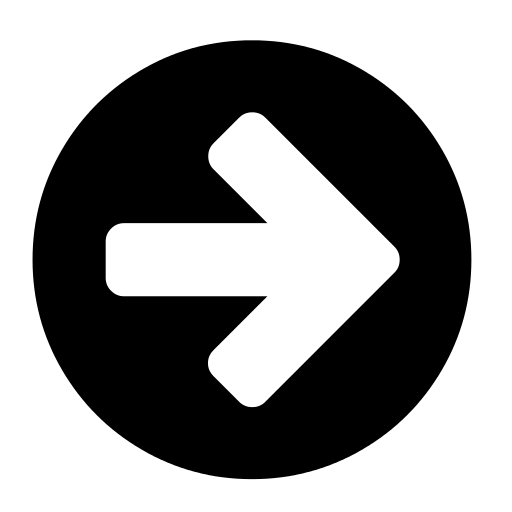
\includegraphics[width=20mm, height=20mm]{./Implementation/Files/arrow.png}
\end{minipage} 	 & \htmlinline{http://commons.wikimedia.org/wiki/File: Circle_arrow_right_font_awesome.svg} \\ \hline

    \begin{minipage}{.5\textwidth}
    
\includegraphics[width=30mm, height=10mm]{./Implementation/Files/volaclogo.jpg}
\end{minipage} 	 & \htmlinline{http://mb.cision.com/Public/3857/ 9287920/93083930d801ade5_800x800ar.jpg} \\ \hline

    \end{tabular}
\end{center}   

\newpage

\section{Code Listing}
\begin{landscape}
%include as many subsections as you have modules
%the code below can be uncommented and used to get a code section from a particular file

\begin{footnotesize}

\newpage
\subsection{Admin Main Program (MainProgram.py)} \label{MP}
\pythonfile[firstline=1]{./Implementation/Files/MainProgram.py}

\newpage
\subsection{Admin Main Menu (AdminMainMenu.py)}\label{AMM}
\pythonfile[firstline=1]{./Implementation/Files/AdminMainMenu.py}

\newpage
\subsection{Admin Database Interface (OpenDatabaseWindow.py)}\label{ODW}
\pythonfile[firstline=1]{./Implementation/Files/OpenDatabaseWindow.py}

\newpage
\subsection{Admin Search Staff Interface (SearchStaffAdmin.py)}\label{SSA}
\pythonfile[firstline=1]{./Implementation/Files/SearchStaffAdmin.py}

\newpage
\subsection{Add Data Window (AddDataGUI.py)}\label{ADGUI}
\pythonfile[firstline=1]{./Implementation/Files/AddDataGUI.py}

\newpage
\subsection{Admin Menubar (MenuBarAdmin.py)}\label{MBA}
\pythonfile[firstline=1]{./Implementation/Files/MenuBarAdmin.py}

\newpage
\subsection{Staff Interface (StaffProgram.py)}\label{SP}
\pythonfile[firstline=1]{./Implementation/Files/StaffProgram.py}

\newpage
\subsection{Staff Menu Bar (StaffMenuBar.py)}\label{SMB}
\pythonfile[firstline=1]{./Implementation/Files/StaffMenuBar.py}

\newpage
\subsection{Manager Main Program (ManagerMainProgram.py)}\label{MMP}
\pythonfile[firstline=1]{./Implementation/Files/ManagerMainProgram.py}

\newpage
\subsection{Manager Main Menu (ManagerMainMenu.py)}\label{MMM}
\pythonfile[firstline=1]{./Implementation/Files/ManagerMainMenu.py}

\newpage
\subsection{Department Information Interface (DepartmentInformation.py)}\label{SI}
\pythonfile[firstline=1]{./Implementation/Files/DepartmentInformation.py}

\newpage
\subsection{Manager - My Information (MyInformation.py)}\label{MI}
\pythonfile[firstline=1]{./Implementation/Files/MyInformation.py}

\newpage
\subsection{Manager Menubar (ManagerMenuBar.py)}\label{MMB}
\pythonfile[firstline=1]{./Implementation/Files/ManagerMenuBar.py}

\newpage
\subsection{Forgotten Account Interface (ForgottenAccount.py)}\label{FA}
\pythonfile[firstline=1]{./Implementation/Files/ForgottenAccount.py}

\newpage
\subsection{Graph Creation (Graph.py)}\label{G}
\pythonfile[firstline=1]{./Implementation/Files/Graph.py}

\newpage
\subsection{Dialog Warning Box (PopupDialog.py)}\label{PPD}
\pythonfile[firstline=1]{./Implementation/Files/PopupDialog.py}

\newpage
\subsection{Calendar (Calender.py)}\label{C}
\pythonfile[firstline=1]{./Implementation/Files/Calender.py}

\newpage
\subsection{Confirm Deletion Dialog (ConfirmDialog.py)}\label{CD}
\pythonfile[firstline=1]{./Implementation/Files/ConfirmDialog.py}

\newpage
\subsection{Report Data Error (Reporterror.py)}\label{RE}
\pythonfile[firstline=1]{./Implementation/Files/Reporterror.py}

\newpage
\subsection{Report Bug (BugReport.py)}\label{BR}
\pythonfile[firstline=1]{./Implementation/Files/BugReport.py}

\newpage
\subsection{Login Window (LoginWindow.py)}\label{LW}
\pythonfile[firstline=1]{./Implementation/Files/LoginWindow.py}

\newpage
\subsection{Add Account Interface (AddingAccounts.py)}\label{AAI}
\pythonfile[firstline=1]{./Implementation/Files/AddingAccounts.py}

\newpage
\subsection{Change Password Interface (ChangePassword.py)}\label{CP}
\pythonfile[firstline=1]{./Implementation/Files/ChangePassword.py}

\newpage
\subsection{CLI to add/edit/remove (EditData.py)}\label{EditData}
\pythonfile[firstline=1]{./Implementation/Files/EditData.py}

\newpage
\subsection{Creating Logins Table (Logins.py)}\label{MMM}
\pythonfile[firstline=1]{./Implementation/Files/Logins.py}


\newpage
\subsection{Creation of the database tables (StaffDatabase.py)}\label{SDB}
\pythonfile[firstline=1]{./Implementation/Files/StaffDatabase.py}

\newpage
\subsection{Creation of the default login details (DefaultLogin.py)}\label{DL}
\pythonfile[firstline=1]{./Implementation/Files/DefaultLogin.py}

\end{footnotesize}

\end{landscape}
